% !TEX root = ../presentation.tex

\begin{frame}{Искажения оптической линзы}
\begin{figure}
\centering
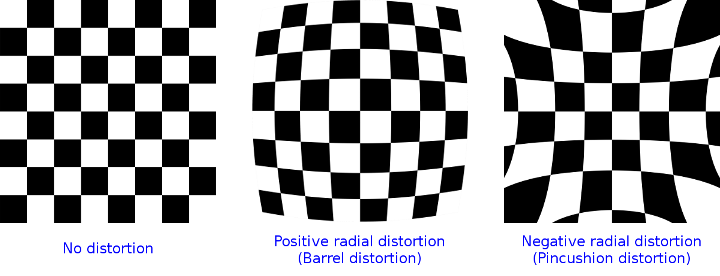
\includegraphics[width=\textwidth]{lens-distortion.png}
\end{figure}
\begin{equation*}
    \label{eq:lens-distortion}
    \begin{split}
        x^{''} = x'(1+k_1r^2 + k_2r^4 + k_3r^6) + 2p_1x^{'}y^{'} + p_2(r^2 + 2x^{'2}) \\ 
        y^{''} = y'(1+k_1r^2 + k_2r^4 + k_3r^6) + 2p_2x^{'}y^{'} + p_1(r^2 + 2y^{'2})
    \end{split}
\end{equation*}
где $k_1$, $k_2$, $k_3$, $p_1$, $p_2$ - коэффициенты дисторции; $r^2 = x^{'2} + y^{'2}$; ($x^{'}, y^{'}$) - координаты проекции точки ($x, y$) в системе координат изображения \textit{при отсутствии дисторции}; ($x^{''}, y^{''}$) - \textit{искаженные} координаты проекции точки ($x, y$) в системе координат изображения.
\end{frame}